\documentclass{article}
\usepackage{amsmath}
\usepackage{graphicx}
\usepackage{biblatex} 
\addbibresource{three_books.bib}

\title{Gaussian Processes and Equivalent Bayesian Linear Regressions}
\author{Douglas Mason}
\date{August 2021}

\begin{document}

\maketitle

\section{Introduction}

Finding the equivalent Bayesian linear regression (BLR) to a Gaussian process (GP) can provide substantial benefits in modeling including (1) it provides potential efficiency savings, (2) it aids interpretability, (3) it is easy to combine multiple models into one. However, while the three major textbooks on the subject \cite{bishop, murphy, rasmussen} cover the subject extensively, it surprised me that they didn't provide a practical side-by-side comparison or recipe for converting the kernel used to generate a GP to an equivalent set of basis functions for a BLR.

Why not remains a mystery to me, but it actually takes a lot of work to get the equivalence just right. This document covers the recipe I arrived at after working through the problem. It is accompanied by a Github repository which can be accessed at https://github.com/KoyoteScience/GP-BLR.


\section{Bayesian Linear Regression}
Bayesian linear regression can be defined by assuming that we can model a predictor as follows:

\begin{equation}
    y=f(\mathbf{x})=\mathbf{\theta}^\top\mathbf{x}
\end{equation} 

given a prior distribution for our model parameters $\boldsymbol{\theta}$ defined as 

\begin{equation}
    \boldsymbol{\theta}_p \sim \mathcal{N}(\mathbf{0},\Sigma_p^{-1})
\end{equation} 

using the convention whereby the normal distribution is defined by two arguments, the means in each dimension and the covariance among the dimensions. Given a set of N observations, over the independent space $x$ and the dependent space $y$, gives us the matrix $X$ of observations in the independent space and the vector $\mathbf{y}$ of corresponding observations in the dependent space.

\begin{equation}
    \Sigma^{-1} = X X^\top + \Sigma_p
\end{equation} 

\begin{equation}
    \boldsymbol{\theta}\sim\mathcal{N}(\Sigma X^\top \mathbf{y} ,\sigma^2\Sigma)
\end{equation} 

where $\sigma$ is the noise parameter, or the square-root of the sum of squared residuals. This gives us

\begin{equation}
    \mathbf{y}\sim\mathcal{N}(X \Sigma X^\top \mathbf{y} ,\sigma^2X^\top\Sigma X)
\end{equation} 


\section{Bayesian Linear Regression with Basis Functions}

We now transform our independent space using a set of basis function $\boldsymbol{\phi}(\mathbf{x})$ and assume that

\begin{equation}
    y_\ast=f(\mathbf{x_\ast})=\boldsymbol{\theta}^\top\boldsymbol{\phi}(\mathbf{x_\ast})
\end{equation} 

Given $N_T$ training samples, $N_\ast$ test samples, and an $N_D$-dimensional basis vector, we arrive at the notation $\Phi=[\boldsymbol{\phi}(\mathbf{x}_0),\boldsymbol{\phi}(\mathbf{x}_1),\dots,\boldsymbol{\phi}(\mathbf{x}_{N_T}))]^\top$, which is a $N_T \times N_D$ matrix, and  $\boldsymbol{\phi}_\ast=\boldsymbol{\phi}(\mathbf{x}_\ast)$, which is a $N_\ast \times N_D$ matrix. This gives us the covariance function:

\begin{equation}
    \Sigma^{-1} = \Phi \Phi^\top + \Sigma_p
\end{equation} 

where we note that the calculation in involves matrix multiplications on the scale $N_D \times (N_T \times N_T) \times N_D + N_D \times N_D$. In other words, we perform a summation (dot product) over the training data points.
Similarly,

\begin{equation}
    \boldsymbol{\theta}\sim\mathcal{N}(\Sigma \Phi^\top \mathbf{y} ,\sigma^2\Sigma)
\end{equation} 

involves matrix multiplations on the scale $N_D \times (N_D \times N_D) \times (N_T \times N_T)$ for the mean, that is, we perform a summation over the basis vector and the training data. We now have model parameters for each $N_D$ dimension in the basis functions. This gives us

\begin{equation}
\label{BLR_posterior}
    \mathbf{y_\ast}(\mathbf{x}_\ast)\sim\mathcal{N}(\boldsymbol{\phi}_\ast\Sigma \Phi^\top\mathbf{y} ,\sigma^2\boldsymbol{\phi}_\ast\Sigma\boldsymbol{\phi}_\ast^\top)
\end{equation} 

with the associated matrix multiplications on the scale $N_\ast \times(N_D \times N_D) \times (N_D \times N_D) \times (N_T \times N_T)$ for the mean and $N_\ast \times (N_D \times N_D) \times (N_D \times N_D) \times N_\ast$ for the covariance. In other words, we most of our summations are over the basis dimensionality $N_D$ and some over the training set dimensionality $N_T$


\section{Gaussian Processes}

The Gaussian Process (GP) is defined differently. Instead of considering a set of multi-valued basis function vectors defined for each point in independent space $\mathbf{x}$, we consider a single-valued function that takes as two points in the independent space as its arguments. This function is the kernel $k(\mathbf{x},\mathbf{x}')$ which can be extrapolated to multiple observations at once as the matrix $K(X,X')$. We thus draw the the associated observations in the dependent space $\mathbf{y}$ according to the normal distribution using the prior distribution:

\begin{equation}
    \begin{bmatrix}
    \mathbf{y} \\
    \mathbf{y_\ast}
    \end{bmatrix} =
    \mathcal{N}\left(\mathbf{0},
    \begin{bmatrix}
    K(X,X) & K(X,X_\ast) \\
    K(X_\ast,X) & K(X_\ast,X_\ast)
    \end{bmatrix}\right)
\end{equation} 

Let us simplify this notation a bit:

\begin{equation}
    \begin{bmatrix}
    \mathbf{y} \\
    \mathbf{y_\ast}
    \end{bmatrix} =
    \mathcal{N}\left(\mathbf{0},
    \begin{bmatrix}
    K & K_\ast \\
    K^\top_\ast & K_{\ast\ast}
    \end{bmatrix}\right)
\end{equation} 

This is a distribution over the observations and the new test points (denoted with the asterisk) jointly. What does it looks like from the new test point's perspective after we account for the observations?  Then we have the posterior distribution:

\begin{equation}
\label{GP_posterior}
\mathbf{y}_\ast\sim\mathcal{N}\left(K_\ast^\top K^{-1}\mathbf{y},K_{\ast\ast}-K_\ast^\top K^{-1}K_\ast \right)
\end{equation}

These calculations require summations in the matrix multiplication at the scale of $N_\ast \times (N_T \times N_T) \times (N_T \times N_T)$ for hte mean and $N_ast \times (N_T \times N_T) \times (N_T \times N_T) \times N_\ast$ for the covariance. In this case, all summations are over the training set dimensionality $N_T$. This the essence of the "kernel trick".

\section{Equating the Bayesian Linear Regression with the Gaussian Process for a Squared-Exponential Kernel}

We can choose any kernel we like for our Gaussian Process prior, and these can be created by performing operations on other kernels, too. We consider the common case of 

\begin{equation}
\label{kernel}
    k_\text{GP}(\mathbf{x},\mathbf{x}') = \exp\left(\frac{(\mathbf{x}'-\mathbf{x})^2}{2l^2}\right) + \sigma_n^2 \delta(\mathbf{x}, \mathbf{x}')
\end{equation}

which is a squared-exponential kernel with white noise added for the variation we expect in repeated measurements at the same point. Note that $l$ defines a length scale for the kernel.
Using the identity 

\begin{equation}
    \int_{-\infty}^{\infty}e^{-a x^2 + b x + c}dx = \sqrt{\frac{\pi}{a}}e^{\frac{b^2}{4a}+c}
\end{equation}

we observe that 

\begin{equation}
    \int_{-\infty}^{\infty}\exp\left(\frac{(x_0-x''_0)^2)}{2l^2}\right)\exp\left(\frac{(x'_0-x''_0)^2)}{2l^2}\right)dx''\propto\exp\left(\frac{x_0-x'_0}{4l^2}\right)
\end{equation}

That is, if we perform an inner product over all possible $x''$s for a basis function defined by a kernel with length scale $l$ at points $x$ and $x'$, this is equivalent to computing a different kernel between $x$ and $x''$. In the case of the squared-exponentianl (gaussian) kernel, the new equivalent kernel has the same form with a length scale that is $\sqrt{2}$ larger.

Looking back at Equations \ref{BLR_posterior} and \ref{GP_posterior}, we can make the following correspondences for the means

\begin{equation}
    \text{mean}(\mathbf{y}_\ast)\sim\boldsymbol{\phi}_\ast \Sigma \Phi^\top \mathbf{y} \sim K_\ast^\top K^{-1} \mathbf{y}
\end{equation}

and the covariances

\begin{equation}
   \text{cov}(\mathbf{y}_\ast) \sim \sigma_n^2\boldsymbol{\phi}_\ast\Sigma\boldsymbol{\phi}_\ast^\top \sim K_{\ast\ast} - K_\ast^\top K^{-1} K_\ast
\end{equation}

The corresponding expressions certainly look similar, but there are noticeable differences. It begs the question, what if there were some kernel $k_\text{BLR}(\mathbf{x},\mathbf{x}')$ that could define a basis set 

\begin{equation}
    \boldsymbol{\phi}(\mathbf{x})=C_N(k_\text{BLR}(\mathbf{x},\mathbf{x_0}),k_\text{BLR}(\mathbf{x},\mathbf{x_1}),\dots,k_\text{BLR}(\mathbf{x},\mathbf{x}_{N_D}))
\end{equation}

with a normalization constant $C_N$ such that the above correspondences could become identities? Note that we also restrict this kernel so that 

\begin{equation}
    C_N^{-1} = \boldsymbol{\phi}^\top(\mathbf{x})\boldsymbol{\phi}(\mathbf{x}) = 1
\end{equation}


Let us set our prior covariance for the Bayesian linear regression to

\begin{equation}
    \Sigma_p=\sigma_n^2 I
\end{equation}

that is, we assume our prior weights have a mean of zero, are uncorrelated, and have a spread in their means identical to the noise of the data we will soon ingest. Let us also set 

\begin{equation}
    k_\text{BLR}(x_0,x'_0)=\exp\left(\frac{x_0-x'_0}{4l^2}\right)
\end{equation}

What we will arrive at is a Bayesian linear regression that produces the same predictions as the Gaussian process regression with kernel

\begin{equation}
    k_\text{GP}(x_0,x'_0)=\exp\left(\frac{x_0-x'_0}{2l^2}\right)
\end{equation}

because the normalization constants will balance each other out, and the model will learn new coefficients for each basis dimension that account for whatever constants haven't been figured out.

Note that in this case, the posterior covariance isn't proportional to $k_\text{GP}$ for the same reason that it isn't proportional to $K_{\ast\ast}$ in Equation \ref{GP_posterior} or $\Sigma_p^{-1}$ in Equation \ref{BLR_posterior}. Rather, if we describe the posterior covariance as a pure kernel function, it would look something like 

\begin{equation}
    \text{cov}(\mathbf{y_\ast})= k_\text{post.}(\mathbf{x}_\ast,\mathbf{x}_\ast) =
    k_\text{equiv.}(\mathbf{x}_\ast,\mathbf{x}) k_\text{equiv.}^\top(\mathbf{x}_\ast,\mathbf{x})
\end{equation}
\begin{equation}
    k_\text{equiv.} = C_N\sigma_n\Sigma^{1/2}k_\text{BLR}^\top(\mathbf{x}_\ast,\mathbf{x})
\end{equation}

which means that inferencing on the posterior mixes up the basis functions defined by $k_\text{BLR}$ according to the operator $\Sigma^{1/2}$, which is defined by performing a summation over the training points (just like with a Gaussian process). What's a little weird about this equation is that it implies our covariance matrix would see its exponents divide by two due to the square root, but because of the identity in Equation 14, it actually multiplies by two. For examples of this basis function set, see Figure \ref{fig:basis}.

\section{Equating the Bayesian Linear Regression with the Gaussian Process for Arbitrary Kernels}

The previous section covered how to accomplish the equivalence between the Bayesian linear regression and the Gaussian process for a squared-exponential kernel for the GP. One take-away was that the equivalent basis in the BLR has a different length scale and prefactor, but since we can just normalize out the prefactosr, all that matters is the different length scale. The other main take-away is that we can use any arbitrary combination of our basis set and the BLR will learn new coefficients to account for that transformation, as evidenced in Equation 24.

The drawback with the previous approach was that, while intuitive, it leaves us in the dark for performing this equivalence for arbitrary kernels. However, we can use the fact that we can use any linear combination of basis functions to achieve the same result. If that's the case, then let's eschew the manual integration and instead define our basis as the eigenvectors of the kernel used in the GP evaluated at the same basis centers used in the previous analysis.

We first calculate our eigenvectors (rows of $V$) and eigenvalues (diagonal elements of $D$) as follows:

\begin{equation}
    VDV^\top = 
    \begin{bmatrix}
    k_\text{GP}(\mathbf{x}_0,\mathbf{x}_0) && k_\text{GP}(\mathbf{x}_0,\mathbf{x}_1) && \dots && k_\text{GP}(\mathbf{x}_0,\mathbf{x}_{N_D}) \\
    k_\text{GP}(\mathbf{x}_1,\mathbf{x}_0) && k_\text{GP}(\mathbf{x}_1,\mathbf{x}_1) && \dots && k_\text{GP}(\mathbf{x}_1,\mathbf{x}_{N_D}) \\
    \vdots && \vdots && \ddots && \vdots \\
    k_\text{GP}(\mathbf{x}_{N_D},\mathbf{x}_0) && k_\text{GP}(\mathbf{x}_{N_D},\mathbf{x}_1) && \dots && k_\text{GP}(\mathbf{x}_{N_D},\mathbf{x}_{N_D}) \\
    \end{bmatrix}
\end{equation}

note that while appearing similar, the right-hand side of Equation 25 is not the same as $K$, which is the kernel evaluated between all training points, but rather the kernel evaluated between all basis centers.

To project our observations into this space, we convolve them with an normalized infinitesimal-width Gaussian kernel, that is, a dirac delta function ($\delta$), but for computational purposes we choose a width that is sufficiently small that it is less than the distance between any two data points to avoid numerical errors. We can perform this projections as follows: 

\begin{equation}
    X_\delta =
    \begin{bmatrix}
    \delta(\mathbf{x}_0,\mathbf{x}_0) && \delta(\mathbf{x}_0,\mathbf{x}_1) && \dots && \delta(\mathbf{x}_0,\mathbf{x}_{N_D}) \\
    \delta(\mathbf{x}_1,\mathbf{x}_0) && \delta(\mathbf{x}_1,\mathbf{x}_1) && \dots && \delta(\mathbf{x}_1,\mathbf{x}_{N_D}) \\
    \vdots && \vdots && \ddots && \vdots \\
    \delta(\mathbf{x}_{N_T},\mathbf{x}_0) && \delta(\mathbf{x}_{N_T},\mathbf{x}_1) && \dots && \delta(\mathbf{x}_{N_T},\mathbf{x}_{N_D}) \\
    \end{bmatrix}
\end{equation}

and then project onto the eigenbasis:

\begin{equation}
    \Phi = X_\delta V
\end{equation}

and similarly for our test data points at $X_\ast$. We then perform the same procedure as for Bayesian linear regression (Equation \ref{BLR_posterior}). For examples of this basis function set, see Figure \ref{fig:basis}.

\begin{figure}
    \begin{center}
    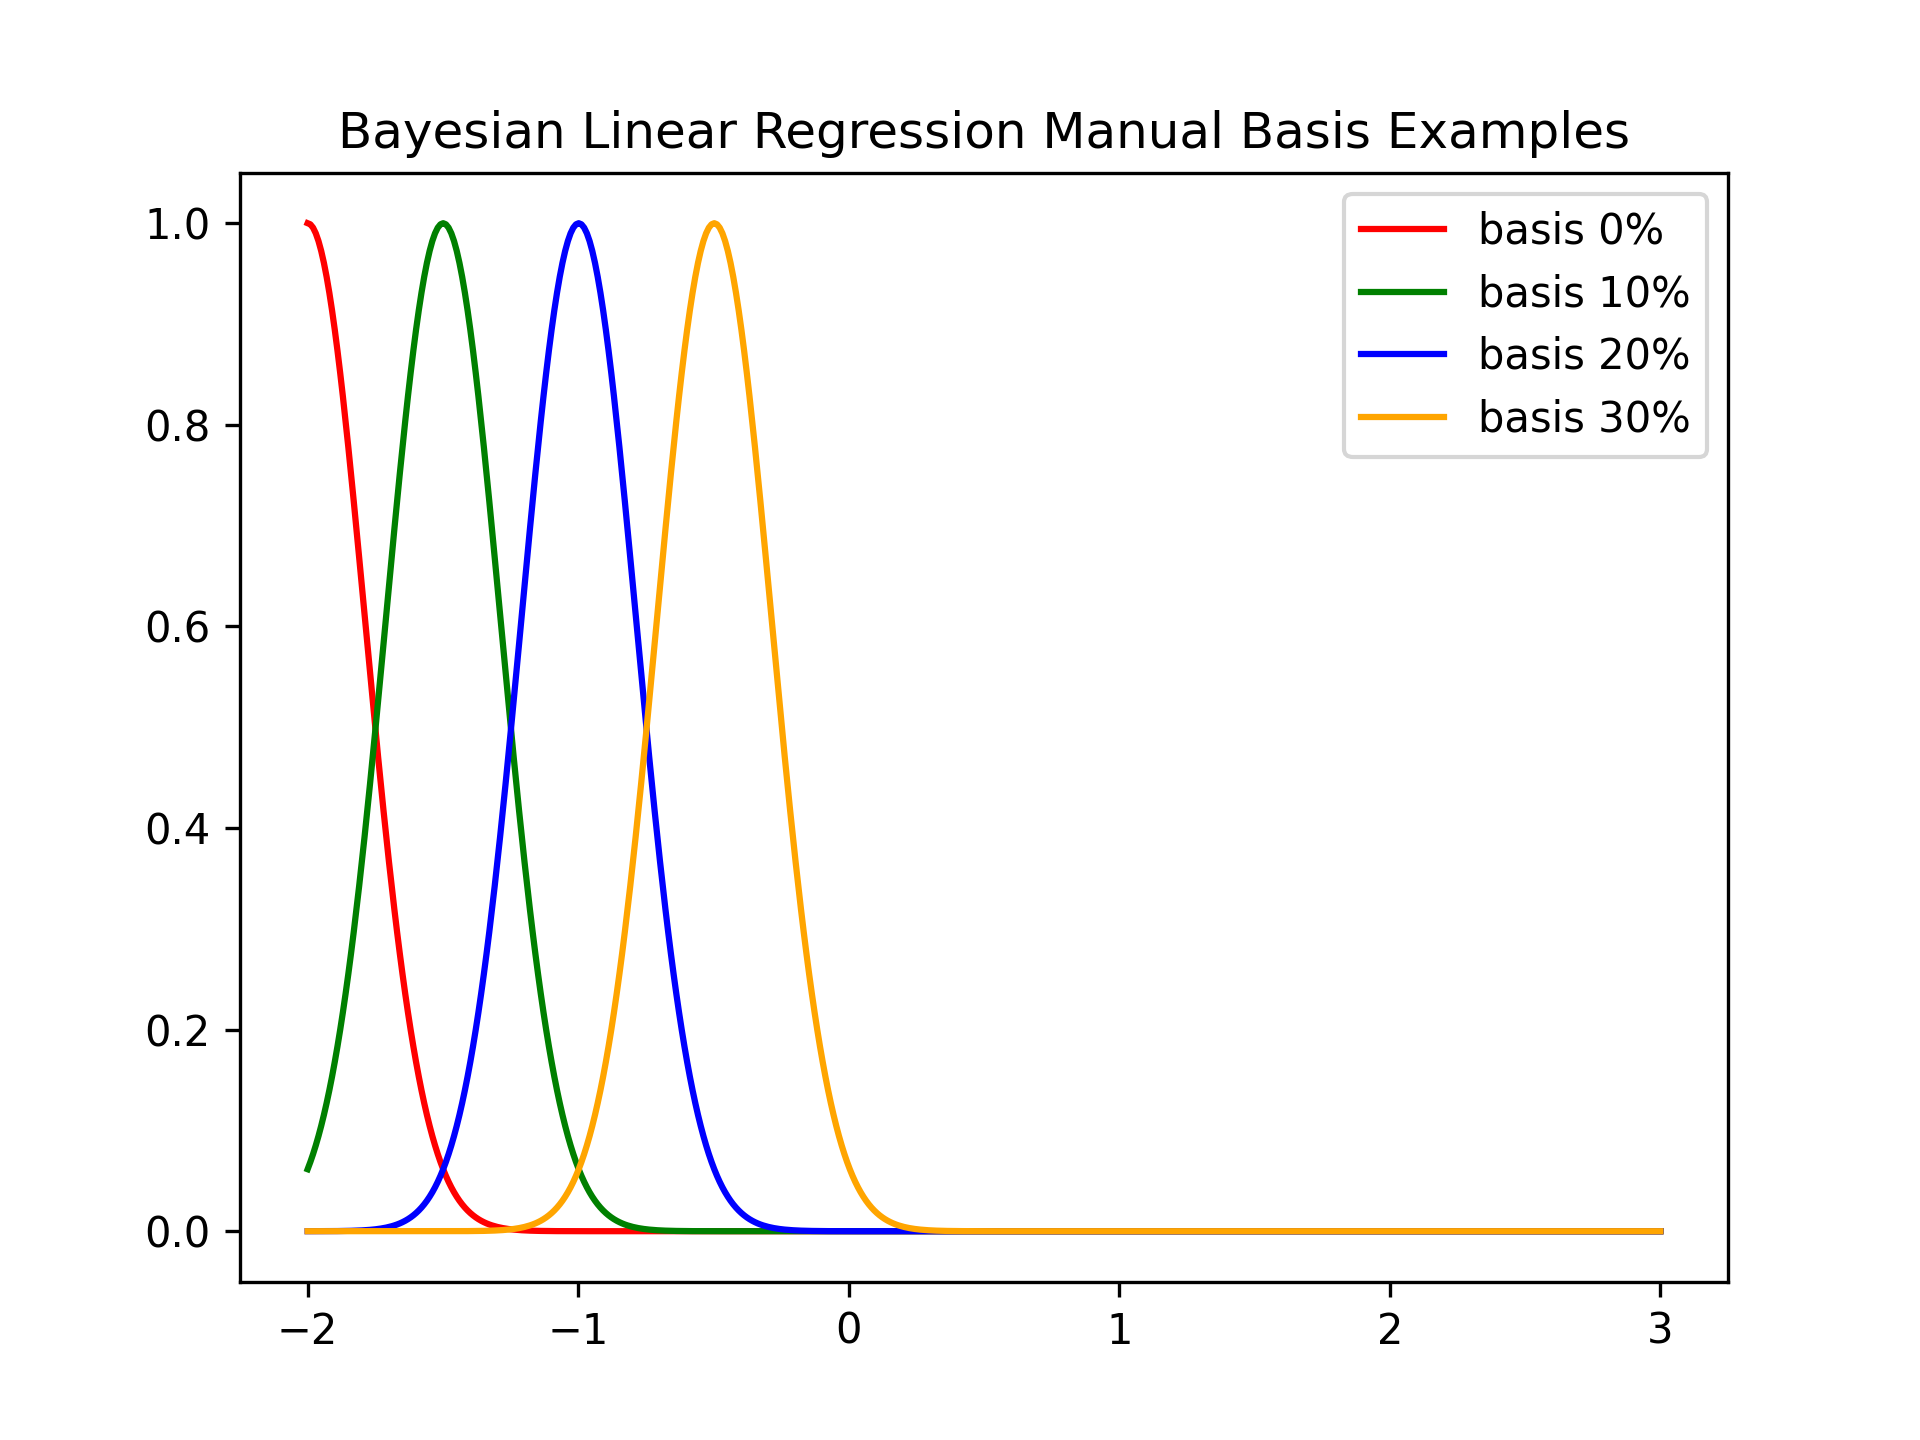
\includegraphics[width=0.75\linewidth]{manualbasis}
    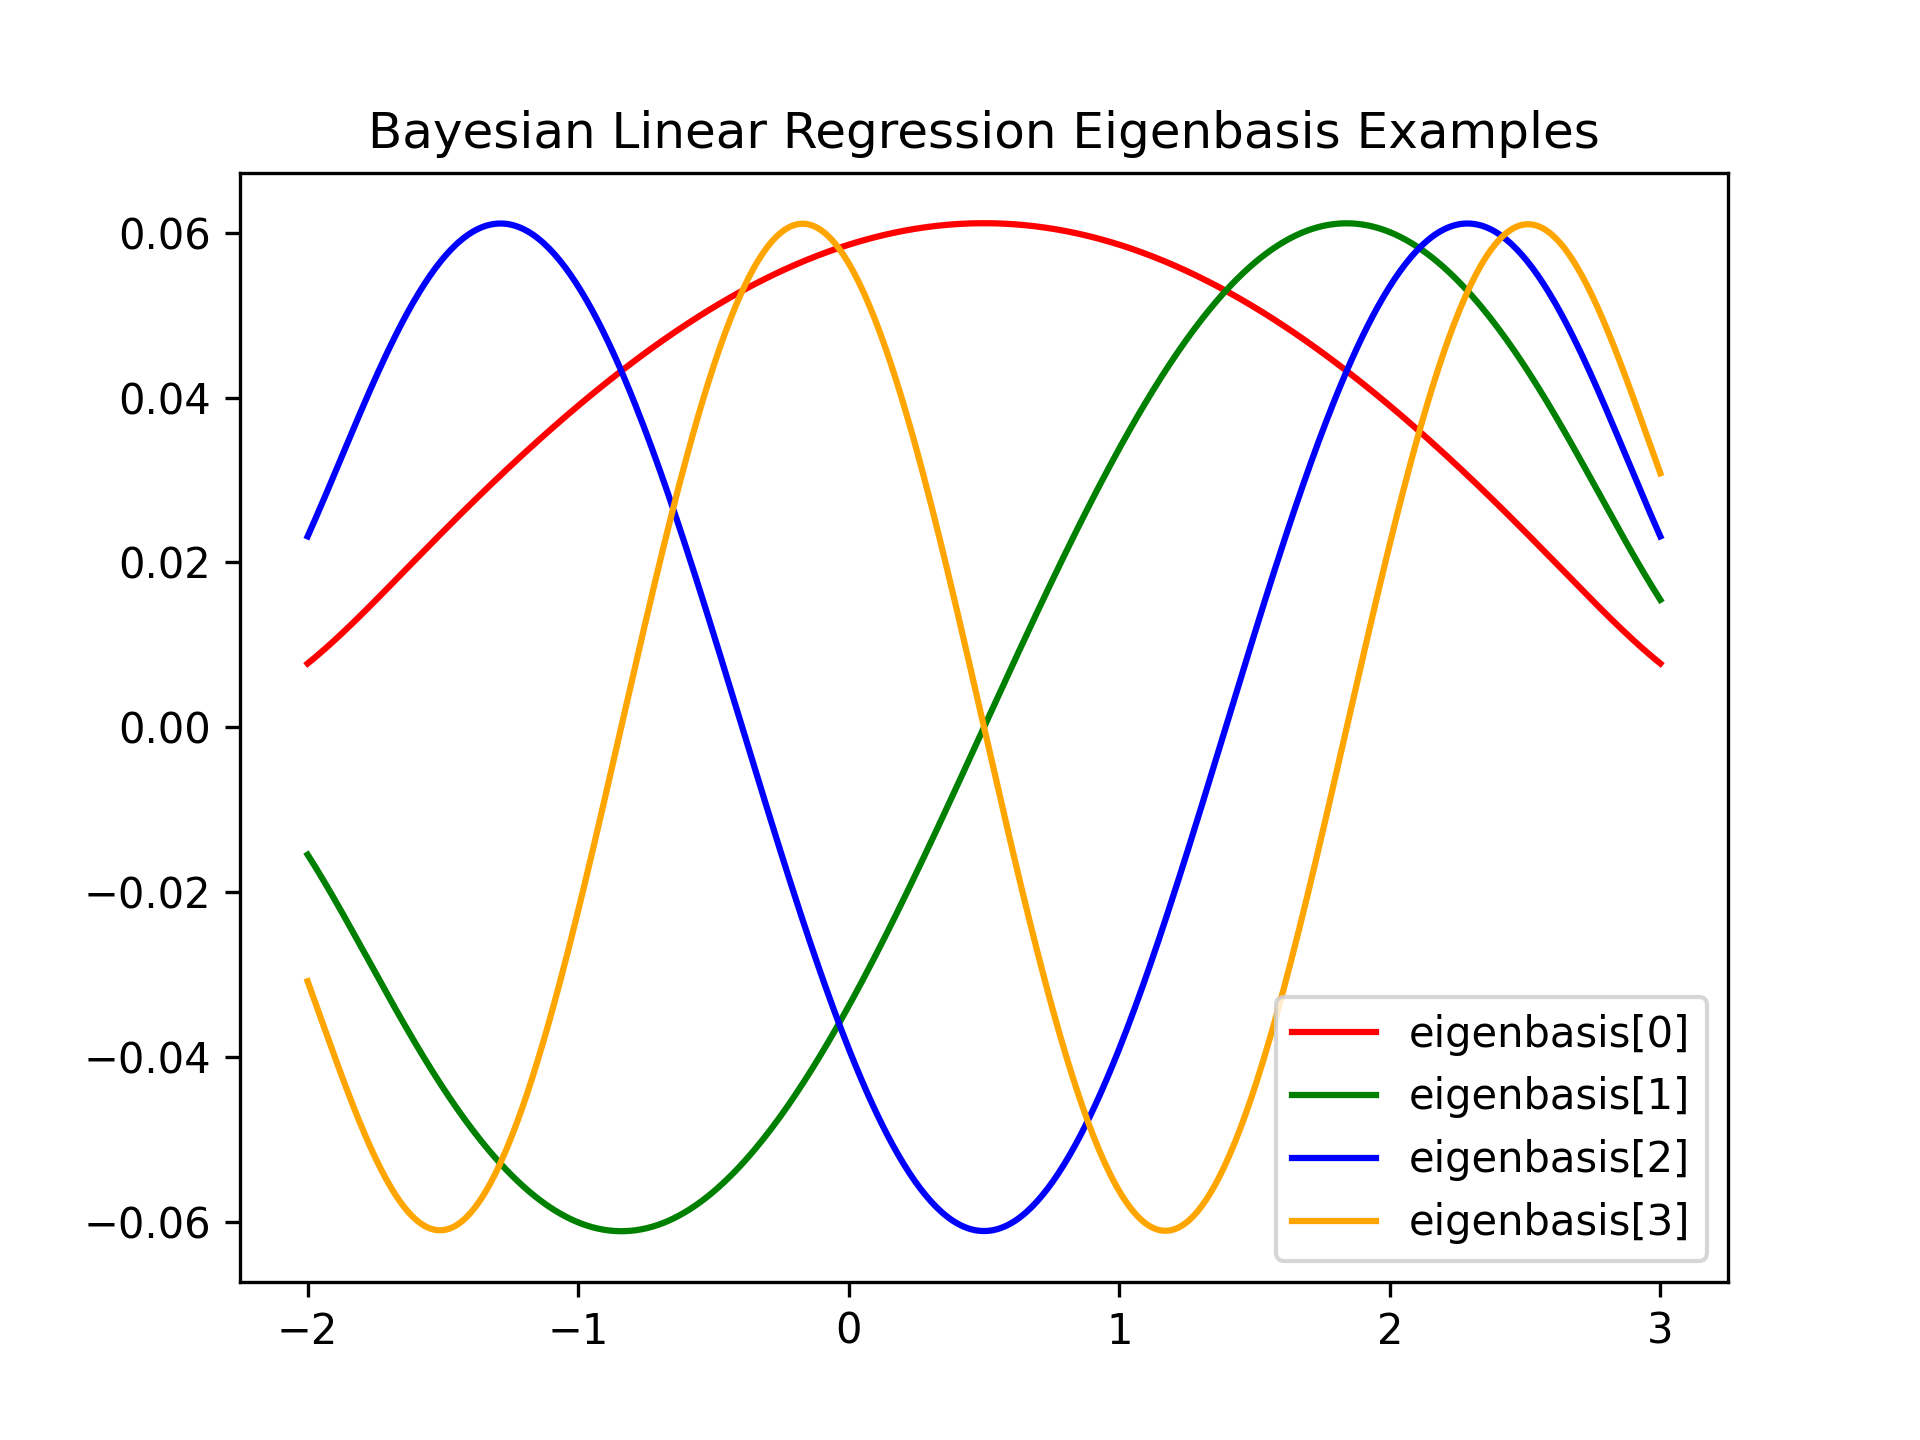
\includegraphics[width=0.75\linewidth]{eigenbasis}
    \caption{Top: The manual basis functions, which are length-scale-adjusted Gaussian distributions, centered at 0\%, 10\%, 20\%, and 30\% along the domain. Bottom: The eigenbasis functions $V$ for the largest four eigenvalues. Note that the sign of each function is arbitrary (can be flipped over the x-axis), and that these functions are the harmonic modes for an equivalent one-dimensional string with fixed endpoints}
    \label{fig:basis}
    \end{center}
\end{figure}

We can perform a couple of simplifications to the procedure outlined in the previous section by considering two ways to reduce the computational complexity: (1) reduce the number of basis centers so that they are spaced according to the length scales of the original kernel and (2) reduce the number of eigenvectors (by filtering out those with small eigenvalues). The first works exceedingly well, except when the variation in the training set y-values is greater than can be afforded by the length scale of the kernel. A GP or equivalent BLR will fit more closely to these widely-varying observations than one with a sparser basis set. Similarly, the second approach loses spatial resolution in proportion to how many eigenvectors are discarded.

Note that just as is the case with the manually-derived basis functions, the BLR will only produce equivalent predictions within the domain that the basis functions cover.




\printbibliography
\end{document}
